% Diese Zeile bitte -nicht- aendern.
\documentclass[course=erap]{aspdoc}

%%%%%%%%%%%%%%%%%%%%%%%%%%%%%%%%%
%% TODO: Ersetzen Sie in den folgenden Zeilen die entsprechenden -Texte-
%% mit den richtigen Werten.
\newcommand{\theGroup}{213} % Beispiel: 42
\newcommand{\theNumber}{A326} % Beispiel: A123
\author{Noah Schlenker \and Leon Baptist Kniffki \and Christian Krinitsin}
\date{Sommersemester 2023} % Beispiel: Wintersemester 2019/20
%%%%%%%%%%%%%%%%%%%%%%%%%%%%%%%%%

% Diese Zeile bitte -nicht- aendern.
\title{Gruppe \theGroup{} -- Abgabe zu Aufgabe \theNumber}

\usepackage{amsfonts}
\usepackage{amsmath}
\begin{document}
\maketitle

\section{Einleitung} \label{sec:einleitung}

Verwendung von Wurzel 2:
\begin{itemize}
  \item Das verhältnis der beiden seitenlängen eines blattes im din-a-format beträgt 1 / sqrt(2) mit rundung auf 
        ganze millimeter. Dadurch ist sichergestellt, dass bei halbierung des blattes entlang der längeren seite wieder 
        ein blatt im din-a-format (mit um eins erhöhter nummerierung) entsteht.
  \item Die wurzel aus 2 ist das frequenzverhältnis zweier töne in der musik bei gleichschwebender stimmung, die einen tritonus, 
        also eine halbe oktave bilden.
  \item In der elektrotechnik enthält die beziehung zwischen scheitelwert und effektivwert von sinusförmiger wechselspannung ebenfalls die konstante 
        sqrt(2).
\end{itemize}

Geschichte über Näherung der Wurzel:
\begin{itemize}
  \item Die alten Inder schätzen $\sqrt{2} \approx \tfrac {577}{408} = 1,414215686$… . Stimmt auf 5 Nachkommastellen. Abweichung beträgt nur +0,0001502 Prozent.
  \item Babylonier aus 1800 v. Chr.: $\tfrac {30547}{21600} = 1,414212962$… . Abweichung von -0,0000424 Prozent.
\end{itemize}

Möglichkeit, $\sqrt{2}$ mit einer unendlichen Präzision zu berechnen. Vorwegnahme: Bignums, Newton-Raphson-Division, Karazuba, Matrixexponentiation. \\
(0,75 Seiten)

\section{Lösungsansatz} \label{sec:loesungsansatz}
\subsection{Big-Num} \label{sec:bignum}
Der Anspruch der Arbeit liegt darin, $\sqrt{2}$ beliebig genau zu berechnen, herkömmliche Variablen mit festgelegter Größe können damit nicht verwendet werden. Hiermit wird die Datenstruktur \textit{Big-Num} eingeführt.
Sie ermöglicht die Darstellung von Zahlen mit beliebiger Größe und Genauigkeit, braucht in C aber eine eigene Implementierung, die im Folgenden erläutert wird. \\
Die Definition der Datenstruktur sieht wie folgt aus:

\begin{lstlisting}
struct bignum {
    uint32_t *digits;
    size_t size;
    size_t fracSize;
};
\end{lstlisting}

Zahlen werden in einem Array von 32-Bit großen \textit{digits} gespeichert. Die Reihenfolge der DoubleWords ist Little-Endian. \textit{Size} gibt die Größe des Arrays an, \textit{fracSize} bestimmt, wie viele Nachkommastellen in dieser Zahl vorhanden sind, dazu mehr
in \ref{sec:newton-raphson}. \\
Nun werden verschiedene Arithmetische Operationen ausgeführt.

\subsubsection*{Addition und Subtraktion}
Bei der Addition und der Subtraktion werden die einzelnen Elemente aufeinander addiert bzw. subtrahiert. Entsteht ein Overflow, wird dieser auf die nächsten Blöcke übertragen. \\
Seien $a$ und $b$ zwei Big-Nums, unterteilt in ihre Blöcke von $0$ bis $m$, so gilt:

\begin{align}
  c &= \sum_{i=0}^m (2^{32i} (a_i + b_i)) \quad  \text{und} \label{eq:bignum_addition} \\ 
  c &= \sum_{i=0}^m (2^{32i} (a_i - b_i)) \,  .          \label{eq:bignum_subtraktion}
\end{align}

Hiermit sind beide Operationen trivial mit einer Laufzeit von $\mathcal{O}(n)$ implementiert.

\subsubsection*{Multiplikation}
Die Multiplikation orientiert sich an der Schulmethode des schriftlichen Multiplizierens. Es wird jeweils ein Block des einen Faktors mit jedem Block des anderen Faktors multipliziert, die Produkte werden aufsummiert.
Dies wird mit jedem Block aus dem ersten Faktoren wiederholt. Mathematisch lässt sich dies mit den eingangs definierten Big-Nums $a$ und $b$ folgendermaßen darstellen:
\begin{equation}
  c = \sum_{i=0}^m (2^{(32i)} b_i \sum_{j=0}^m a_j) \, .
\end{equation}

Damit funktioniert auch die triviale Multiplikation mit einer Laufzeit von $\mathcal{O}(n^2)$. Im Folgenden wird ein Algorithmus zur schnelleren Berechnung des Produkts erläutert.

\subsection{Karazuba-Multiplikation} \label{sec:karazuba}
Erklärung des Algorithmus und der Umsetzung im Code. \\
(0,75 Seiten)

\subsection{Schnelle Exponentiation} \label{sec:schnelle_exponentiation}
Die schnelle Exponentiation nutzt Assoziativität und Potenzgesetze, um die Zahl der der Multiplikationen bei der Exponentiation von $\mathcal{O}(n)$ auf $\mathcal{O}(\log{}n)$ zu verringern. 
Naiv kann eine Potenz $a^n$ mit $n\in\mathbb{N}$ nach der Schulmethode mit \(\prod_{1}^{n} a \) berechnet werden. Dafür benötigt man allerdings $n-1$ Multiplikationen, was bei großen Werten für $n$ zu einer langen Berechnung ausartet.\\
Um dieses Problem effizienter zu lösen, werfen wir erst einmal einen Blick auf die Potenzgesetze für assoziative Operatoren. Denn sowohl eine Multiplikation, als auch eine Addition im Exponenten kann aufgeteilt werden:
\begin{equation}\label{exponenten_addition}
    a^{n+m} = a^n * a^m
\end{equation}
\begin{equation}\label{exponenten_multiplikation}
    a^{n*m} = (a^n)^{^m}
\end{equation}
Wenn man also $a^n$ und $a^m$ effizienter als mit $n+m$ Multiplikationen berechnen kann, kann man auch $a^{n+m}$ mit \ref{exponenten_addition} effizient berechnen.\\
Bei der schnellen Exponentiation berechnet man durch wiederholtes Quadrieren alle $a^{(2^k)}$ mit $2^k \le n$. Denn nach \ref{exponenten_multiplikation} gilt:
\[ {\left( a^{(2^k)} \right)}^2 = a^{(2^k*2)} = a^{(2^{k+1})}.\]
Um $a^n$ mit $n=2^k$ zu berechnen, sind damit nur noch $k=\log_2n$ Multiplikationen notwendig.
\\Potenzen mit der Form $a^{(2^k)}$ können also effizient berechnet werden, um nun auch Potenzen mit $n\in\mathbb{N}$ berechnen zu können, nutzt man \ref{exponenten_addition}. 
Jede Zahl $n\in\mathbb{N}$ kann durch Addition von Zweierpotenzen dargestellt werden (Binärsystem). \\
Sei $n$ in Binärdarstellung $b_0*2^0+b_1*2^1+b_2*2^2\dots$, so erhält man $a^n$ mit:
\[ a^n = a^{b_0*2^0+b_1*2^1+b_2*2^2\dots} = a^{b_0*2^0} * a^{b_1*2^1} * a^{b_2*2^2} \dots \]
Da $b_i$ nur die Werte $0$ und $1$ annehmen kann, ist es am Ende eine boolsche Entscheidung, ob der aktuelle Wert von $a^{(2^k)}$ auf das Zwischenergebnis aufmultipliziert wird, oder nicht.\\
Außerdem gilt:
\begin{equation}\label{swap_exponents}
      a^n*a^m = a^m*a^n
\end{equation}
Auch wenn diese Gleichung auf den ersten Blick nach Kommutativität aussieht, gilt sie aufgrund der Assozitivität in Gruppen, da nur die Klammerung geändert wird:
\[ \overbrace{(a*\dots*a)}^n*\overbrace{(a*\dots*a)}^m = \overbrace{(a*\dots*a)}^m*\overbrace{(a*\dots*a)}^n \]
Ein Beispiel:
\[ 7^3*7^4 = \overbrace{(7*7*7)}^3*\overbrace{(7*7*7*7)}^4 = \overbrace{(7*7*7*7)}^4*\overbrace{(7*7*7)}^3 = 7^4*7^3 \]
Demnach macht es keinen Unterschied, ob zuerst $a^{(2^k)}$ mit dem kleinsten oder dem größten $k$ aufmultipliziert wird.\\
Da $(\mathbb{N}^{2\times 2}, *)$ eine Gruppe und damit assoziativ ist, kann die schnelle Exponentiation auch für das lösen von $a\in\mathbb{N}^{2\times 2}$ genutzt werden.

\subsection{Matrizen} \label{sec:matrizen}
anwendung der schnellen exponentiation auf matrizen, beispiel dazu
(0.75 Seiten)

\newpage
\subsection{Newton-Raphson-Division} \label{sec:newton-raphson}
Mithilfe der bereitgestellten Matrix werden nun die Werte ausgerechnet, die bei der Division an $\sqrt{2}$ konvergieren.
Nun beschäftigen wir uns mit der Darstellung von Kommazahlen und einem Algorithmus zur Berechnung eines Quotienten in dieser Darstellung. \\
Wir kennen zwei verschiedene Formen der Darstellung von Kommazahlen: Fließkommazahlen nach \textit{IEEE-754} und Fixpunktzahlen.
Der Vorteil von Fließkommazahlen ist ihr großer Wertebereich, der dafür mit schwankender Genauigkeit einherkommt, wie man in Abbildung \ref{img:fließkommazahlen-wertebereich} erkennen kann.

\begin{figure}[h] \centering
  \includegraphics[scale=0.35]{graphiken/fließkommazahlen-wertebereich.png} 
  \caption{Exakt darstellbare Fließkommazahlen mit verschiedenen Mantissen (Entnommen aus \cite{fliesskommazahlen})} \label{img:fließkommazahlen-wertebereich}
\end{figure} 

Fixpunktzahlen haben einen kleineren Wertebereich bei gleichem Speicherverbrauch, besitzen dafür eine schnellere und deutlich einfachere Arithmetik und haben eine gleichbleibene Genauigkeit im gesamten Wertebereich - zu sehen in Abbildung \ref{img:fixpunktzahlen-wertebereich}.

\begin{figure}[h] \centering
  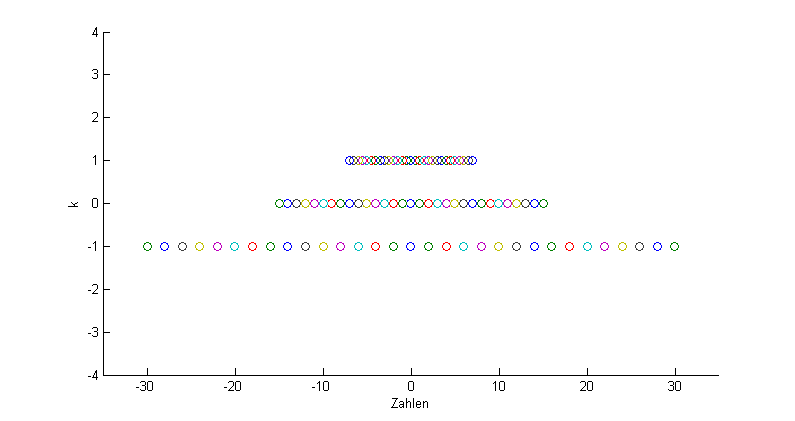
\includegraphics[scale=0.4]{graphiken/fixpunktzahlen-wertebereich.png} 
  \caption{Exakt darstellbare Fixpunktzahlen mit k Nachkommastellen (Entnommen aus \cite{fixpunktzahlen})} \label{img:fixpunktzahlen-wertebereich}
\end{figure} 

Ein weiterer Vorteil von Fixpunktzahlen liegt darin, dass man unendlich viele Nachkommastellen einfach darstellen kann, in dem man beispielsweise die implementierten Big-Nums aus \ref{sec:bignum} verwendet. Aus den
genannten Gründen lässt sich schließen, dass sich die Nutzung von Fixpunktzahlen viel besser eignet, um $\sqrt{2}$ mit beliebig vielen Nachkommastellen darzustellen. \\

Die Newton-Raphson-Division ist ein Algorithmus zur Berechnung der Division. Er nutzt das Newton-Verfahren, das dafür da ist, Nullstellen von Funktionen zu approximieren und wendet dies so an, um Quotienten zu berechnen. 
Das Verfahren besteht aus 3 Schritten, die nun erläutert werden \cite{newton_raphson_division}. Wir wollen den Quotienten aus $a$ und $b$ berechen, mit $a, b \in \mathbb{N}$. \\
Zunächst brauchen wir eine erste Näherung. Wir bitshiften den Quotienten so lange nach rechts, bis $0,5 \leq b < 1,0$. Die erste Näherung erhalten wir mit:
\begin{equation} \label{eq:erste_naeherung}
  x_0 = \frac{48}{17} - b \frac{32}{17} \, .
\end{equation}

Als Nächstes berechnen wir iterativ immer bessere Näherungen:
\begin{equation} \label{eq:iterationen}
  x_{i + 1} = x_i (2 - b x_i) \, .
\end{equation}
Mit jeder Iteration erhält das Ergebnis doppelt so viele Nachkommastellen wie vorher, es wird auch doppelt so genau. Um die Anzahl der benötigten Iterationen zu erhalten, betrachten wir folgende Formel, wobei k für die erwartete Anzahl an Nachkommastellen im Ergebnis steht:
\begin{equation} \label{eq:anzahl_iterationen}
  \text{Iterationen} = \lfloor log_2k\rfloor \, .
\end{equation}

Um nun das Endergebnis zu erhalten, multiplizieren das Zwischenergebnis mit $a$ und erhalten somit unser Ergebnis der Division.
Es kann passieren, dass durch die ständige Verdoppelung der Nachkommastellen, die Zahl zu viele davon besitzt als notwendig. Diese Ziffern werden einfach abgeschnitten. \\
Als illustratives Beispiel berechnen wir $5 / 12$ mit sieben Nachkommastellen. Die Anzahl der Iterationen beträgt $ \lfloor log_27\rfloor = 2$.
Nach wiederholten bitshiften der Zahl $12$ erhalten wir $(0,1100)_2 = (0,75)_{10}$. Wir berechnen die Zwischenschritte:
\begin{align}
  x_0 &= (10,1101.001)_2 - (0,1100)_2 \cdot (1,111)_2 = (1,0110.101)_2 \,; \label{eq:beispiel_x0} \nonumber \\ 
  x_1 &= (1,0110.101)_2 \cdot (2_{10} - (0,1100)_2 \cdot (1,0110.101)_2) = (1,0101.0100.0001.0101.00)_2  \,; \label{eq:beispiel_x1} \nonumber \\
  x_2 &= (1,0101.0100.0001.0101.00)_2 \cdot (2_{10} - (0,1100)_2 \cdot (1,0101.0100.0001.0101.00)_2) \nonumber \\ 
      &= (1,0101.0101.0101.0100.0010.1000.1011.0101.0100.0000)_2 \,. \label{eq:beispiel_x2} \nonumber
\end{align}
Multipliziert man $x_2$ mit dem geshifteten $a = (0,0101)_2$ und shiftet dieses so weit, so dass die Zahl nur noch sieben Nachkommastellen besitzt, erhält man das
Ergebnis $(0,0110.101)_2 = (0,4141)_{10}$, welches sich an der dritten dezimalen Nachkommastelle vom eigentlichen Ergebnis $0,41\overline{6}$ abweicht. \\

Wir sind in der Lage, Divisionen durchzuführen und effizient Werte auszurechnen, die das Ergebnis approximieren.

(1 Seite gedacht, jetzt 2)

% TODO: Je nach Aufgabenstellung einen der Begriffe wählen
\section{Genauigkeit} \label{sec:genauigkeit}
Wahrscheinlich Genauigkeit, da es die Aufgabe ist, $\sqrt{2}$ beliebig genau darzustellen. \\

Umfangreiche Erklärung darüber, wie die Matrix Elemente an $\sqrt{2}$ konvergiert und Newton-Raphson and die Division. Erklärung, wie die Kombination aus Bignum und Fixkommazahlen unendliche Genauigkeit 
ermöglicht, auf Kosten von Laufzeit, die im nächsten Kapitel beleuchtet wird. \\ 
(1,5 - 2 Seiten?)

\section{Performanzanalyse} \label{sec:performanz}
Newton Raphson Laufzeit erklären, mit Graphiken demonstrieren, das selbe mit Exponentiation. \\
Vergleichsimplementierungen ansetzen (SIMD, nicht SIMD? / Karazuba, normale Multiplikation / Bitshifts?), Graphisch laufzeiten vergleichen, tatsächliche Performanz erklären und schlussfolgern. \\
(2 - 3 Seiten)

\section{Zusammenfassung und Ausblick} \label{sec:zusammenfassung}
Ziel erreicht, unendliche Präzision ist gegeben. Nutzer können, abhängig von ihren Anforderungen oder "Computerspezifikationen", die Wurzel von 2 mit diesem Programm berechnen. \\
Ausblick: SIMD in AVX, mithilfe von 256 Bit kann man Multiplikationen noch schneller machen. Division lässt sich wahrscheinlich nicht optimieren, da SIMD nicht verwendet werden kann, 
und immer eine gewisse Anzahl an Iterationen gebraucht wird. \\
(0,75 - 1 Seite) \\
(Insgesamt 6 - 7,75 Seiten, 2 - 4 Seiten fehlen!)

% TODO: Fuegen Sie Ihre Quellen der Datei Ausarbeitung.bib hinzu
% Referenzieren Sie diese dann mit \cite{}.
% Beispiel: CR2 ist ein Register der x86-Architektur~\cite{intel2017man}.
\bibliographystyle{plain}
\bibliography{Ausarbeitung}{}

\end{document}
